\documentclass{beamer}
\usepackage[utf8]{inputenc}
\usepackage[T1]{fontenc}
% \usepackage{amscd, amsfonts, amsmath, amssymb, amstext, amsthm, caption, epsfig, fancyhdr, float, graphicx, latexsym, mathtools, multicol, multirow, algorithm, chngcntr}
\usepackage[english]{babel}
\usepackage{booktabs}

\usepackage{amsmath,amssymb}
\usepackage{graphicx}
\usepackage{caption}
\usepackage{subfig}
\usepackage{xspace}
\usepackage{fourier}

\usepackage{tikz}
\usetikzlibrary{shapes,arrows}
\usepackage{tkz-graph}
\usetikzlibrary{automata,arrows,positioning,calc}
\usetikzlibrary{positioning}
\usetikzlibrary{fit}
\usetikzlibrary{backgrounds}
\usetikzlibrary{calc}
\usetikzlibrary{shapes}
\usetikzlibrary{mindmap}
\usetikzlibrary{decorations.text}
\usetikzlibrary{snakes}

% \theoremstyle{definition} % insert bellow all blocks you want in normal text
% \newtheorem{definition}{Definition}



% tikzmark command, for shading over items
\newcommand{\tikzmark}[1]{\tikz[overlay,remember picture] \node (#1) {};}
% Define block styles
\tikzstyle{decision} = [diamond, draw, fill=blue!20,
    text width=4.5em, text badly centered, node distance=3cm, inner sep=0pt]
\tikzstyle{block} = [rectangle, draw, fill=blue!20,
    text width=5em, text centered, rounded corners]
\tikzstyle{line} = [draw]
\tikzstyle{cloud} = [draw, ellipse,fill=red!20, node distance=3cm,
    minimum height=2em]

\usepackage[most]{tcolorbox}

\setbeamertemplate{blocks}[rounded][shadow=true] % use rounded blocks with standard beamer shadow


% Distributions.
\newcommand*{\UnifDist}{\mathsf{Unif}}
\newcommand*{\ExpDist}{\mathsf{Exp}}
\newcommand*{\DepExpDist}{\mathsf{DepExp}}
\newcommand*{\GammaDist}{\mathsf{Gamma}}
\newcommand*{\LognormalDist}{\mathsf{LogNorm}}
\newcommand*{\WeibullDist}{\mathsf{Weib}}
\newcommand*{\ParetoDist}{\mathsf{Par}}
\newcommand*{\NormalDist}{\mathsf{Norm}}

\newcommand*{\GeometricDist}{\mathsf{Geom}}
\newcommand*{\NegBinomialDist}{\mathsf{NegBin}}
\newcommand*{\PoissonDist}{\mathsf{Poisson}}
\newcommand*{\BivariatePoissonDist}{\mathsf{BPoisson}}
\newcommand*{\CyclicalPoissonDist}{\mathsf{CPoisson}}

\newcommand*{\iid}{\textbf{iid}\@\xspace}
\newcommand*{\pdf}{\textbf{pdf}\@\xspace}
\newcommand*{\cdf}{\textbf{cdf}\@\xspace}
\newcommand*{\pmf}{\textbf{pmf}\@\xspace}
\newcommand*{\abc}{{\textbf{abc}}\@\xspace}
\newcommand*{\smc}{\textbf{smc}\@\xspace}
\newcommand*{\mcmc}{\textbf{mcmc}\@\xspace}
\newcommand*{\ess}{\textbf{ess}\@\xspace}
\newcommand*{\mle}{\textbf{mle}\@\xspace}
\newcommand*{\bic}{\textbf{bic}\@\xspace}
\newcommand*{\kde}{\textbf{kde}\@\xspace}
\newcommand*{\glm}{\textbf{glm}\@\xspace}
\newcommand*{\xol}{\textbf{xol}\@\xspace}
\newcommand*{\cpu}{\textbf{cpu}\@\xspace}
\newcommand*{\gpu}{\textbf{gpu}\@\xspace}
\newcommand*{\arm}{\textbf{arm}\@\xspace}

\def \si {\sigma}
\def \la {\lambda}
\def \al {\alpha}
% \def\e*{\end{eqnarray*}}
\def \di{\displaystyle}

\def \E{\mathbb E}
\def \N{\mathbb N}
\def \Z{\mathbb Z}
\def \NZ{\mathbb{N}_0}
\def \I{\mathbb I}
\def \w{\widehat}
\def \P {\mathbb P}
\def \V{\mathbb V}


\newcommand{\CL}{\mathbb{C}}
\newcommand{\RL}{\mathbb{R}}
\newcommand{\nat}{{\mathbb N}}
\newcommand{\Laplace}{\mathscr{L}}
\newcommand{\e}{\mathrm{e}}
\newcommand{\ve}{\bm{\mathrm{e}}} % vector e

\renewcommand{\L}{\mathcal{L}} % e.g. L^2 loss.

\newcommand{\ih}{\mathrm{i}}
\newcommand{\oh}{{\mathrm{o}}}
\newcommand{\Oh}{{\mathcal{O}}}
\newcommand{\Exp}{\mathbb{E}}

\newcommand{\Norm}{\mathcal{N}}
\newcommand{\LN}{\mathcal{LN}}
\newcommand{\SLN}{\mathcal{SLN}}

\renewcommand{\Pr}{\mathbb{P}}
\newcommand{\Ind}{\mathbb I}
\newcommand\bfsigma{\bm{\sigma}}
\newcommand\bfSigma{\bm{\Sigma}}
\newcommand\bfLambda{\bm{\Lambda}}
\newcommand{\stimes}{{\times}}
\def \limsup{\underset{n\rightarrow+\infty}{\overline{\lim}}}
\def \liminf{\underset{n\rightarrow+\infty}{\underline{\lim}}}




% vertical separator macro
\newcommand{\vsep}{
  \column{0.0\textwidth}
    
\begin{tikzpicture}
      \draw[very thick,black!10] (0,0) -- (0,7.3);
    \end{tikzpicture}
}
\newcommand\blfootnote[1]{%
  \begingroup
  \renewcommand\thefootnote{}\footnote{#1}%
  \addtocounter{footnote}{-1}%
  \endgroup
}

% More space between lines in align
% \setlength{\mathindent}{0pt}

% Beamer theme
\usetheme{ZMBZFMK}
\usefonttheme[onlysmall]{structurebold}
\mode<presentation>
\setbeamercovered{transparent=10}

% align spacing
\setlength{\jot}{0pt}

\setbeamertemplate{navigation symbols}{}%remove navigation symbols

\title[BLOCKASTICS]{Blockchain miner's risk management}
\author{Pierre-O. Goffard}
\institute[UNISTRA]{Université de Strasbourg\\
 \texttt{goffard@unistra.fr}
}
\date{\today}
% \titlegraphic{\includegraphics[width=2.5cm]{../../Figures/bfs_logo.png}} 

\begin{document}
\begin{frame}
  \titlepage
\end{frame}
\begin{frame}
  \tableofcontents
\end{frame}

\section{PoW Blockchain}
\begin{frame}{Blockchain}
A decentralized data ledger made of blocks maintained by achieving consensus in a P2P network.
\begin{columns}
\begin{column}{0.5\textwidth}
% \small

\begin{itemize}
  \item Decentralized
  \item Public/private
  \item Permissionned/permissionless
  \item Immutable
  \item Incentive compatible
\end{itemize}
\end{column}
\begin{column}{0.5\textwidth}
\begin{center}
\begin{tikzpicture}[-, >=stealth', auto, semithick, node distance=01cm]
\tikzstyle{every edge}=[snake=expanding waves,segment length=1mm,segment angle=10, draw]

\tikzstyle{full node}=[circle, fill=tublue,draw=tublue,thick,text=black,scale=0.8]
\tikzstyle{light node}=[circle, fill=white,draw=tublue,thick,text=black,scale=0.8]
\node[full node]    (1)                     {};
\node[full node]    (2)[above right of=1]         {};
\node[full node]    (3)[above left of=1]         {};
\node[full node]    (4)[below of=1]         {};
\node[full node]    (5)[right of=4]         {};
\node[full node]    (6)[below of=4]         {};
\node[light node]    (7)[left of=1]         {};
\node[light node]    (8)[right of=2]         {};
\node[light node]    (9)[left of=4]         {};
\node[light node]    (10)[above right of=5]         {};
\node[light node]    (11)[ right of=5]         {};
\node[light node]    (12)[ below right of=5]         {};
% \node[light node]    (4)[above of=2]         {};
\path

(1) edge node{} (2)
    edge node{} (3)
    edge node{} (7)
    ;
\path
(5) edge node{} (10)
    edge node{} (11)
    edge node{} (12)
    ;
    \path
(4) edge node{} (5)
    edge node{} (1)
    edge node{} (9)
    edge node{} (6)
    ;
    \path
(2) edge node{} (8)   
    ;
\end{tikzpicture}
\end{center}
\end{column}
\end{columns}

\vspace{0.2cm}
\begin{tcolorbox}[enhanced,drop shadow, title=Focus of the talk]
Public and permissionless blockchain equipped with the Proof-of-Work protocol.
\end{tcolorbox}
\end{frame}

% \begin{frame}{Consensus protocols}
% The mechanism to make all the nodes agree on a common data history.\\
% \vspace{0.3cm}
% The three dimensions of blockchain systems analysis
% \begin{enumerate}
%   \item Efficiency
%   \begin{itemize}
%     \item Throughputs
%     \item Transaction confirmation time
%   \end{itemize}
%   \item Decentralization
%   \begin{itemize}
%     \item Fair distribution of the accounting right
%   \end{itemize}
%   \item Security 
%   \begin{itemize}
%     \item Resistance to attacks
%   \end{itemize}
% \end{enumerate}
% \footnotesize
% % \begin{thebibliography}{1}
% % \bibitem{Fu2020}
% % X.~Fu, H.~Wang, and P.~Shi, ``A survey of blockchain consensus algorithms:
% %   mechanism, design and applications,'' {\em Science China Information
% %   Sciences}, vol.~64, nov 2020.
% % \end{thebibliography}
% \blfootnote{\url{https://pierre-olivier.goffard.me/BLOCKASTICS/}}
% \end{frame}
\begin{frame}{Applications of blockchain: Cryptocurrency}
\begin{columns}
\begin{column}{0.5\textwidth}
   
{\footnotesize
\begin{thebibliography}{1}
\bibitem{Na08}
S.~Nakamoto, ``Bitcoin: A peer-to-peer electronic cash system.'' Available at
  \href{https://bitcoin.org/bitcoin.pdf}{https://bitcoin.org/bitcoin.pdf},
  2008.
\end{thebibliography}  
}
\end{column}
\begin{column}{0.5\textwidth}  %%<--- here
    \begin{center}
     
\includegraphics[width=0.5\textwidth]{../../Figures/bitcoin-6284869_1920.png}
     \end{center}
\end{column}
\end{columns}

\begin{itemize}
  \item Transaction anonymity
  \item No need for a thrusted third party
\end{itemize}
\end{frame}
% \begin{frame}{Decentralized finance}
% DEFI creates new financial architecture
% \begin{columns}
% \begin{column}{0.5\textwidth}
% \begin{itemize}
% \item[+] Non custodial
% \item[+] Anonymous
% \item[+] Permisionless
% \item[+] openly auditable
% \end{itemize}
% \end{column}
% \begin{column}{0.5\textwidth} 
% \begin{itemize}
% \item[-] Unregulated
% \item[-] Tax evasion
% \item[-] Fraud
% \item[-] Money laundering
% \end{itemize} 
% \end{column}
% \end{columns}
% \vspace{0.5cm}
% Extends the Bitcoin promises to more complex financial operations
% \begin{itemize}
%   \item Collateralized lending
%   \item Decentralized Exchange Platform
%   \item Tokenized assets
%   \item Fundraising vehicle (ICO, STO, ...)
% \end{itemize}
% \vspace{0.3cm}
% \scriptsize
% \begin{thebibliography}{1}

% \bibitem{werner2021sok}
% S.~M. Werner, D.~Perez, L.~Gudgeon, A.~Klages-Mundt, D.~Harz, and W.~J.
%   Knottenbelt, ``Sok: Decentralized finance (defi),'' 2021.

% \end{thebibliography}

% \end{frame}
\begin{frame}{What's inside a block?}
A block consists of 
\begin{itemize}
\item a header 
\item a list of "transactions" that represents the information recorded through the blockchain. 
\end{itemize}
The header usually includes 
\begin{itemize}
\item the date and time of creation of the block, 
\item the block height which is the index inside the blockchain, 
\item the hash of the block 
\item the hash of the previous block. 
\end{itemize}
\begin{tcolorbox}[enhanced,drop shadow, title=Question]
What is the hash of a block?
\end{tcolorbox}
\end{frame}
\begin{frame}{Cryptographic Hash function}
\small
A function that maps data of arbitratry size (message) to a bit array of fixed size (hash value)
$$
h:\{0,1\}^\ast\mapsto \{0,1\}^d. 
$$
A good hash function is
\begin{itemize}
\item deterministic
\item quick to compute
\item One way
\begin{itemize}
  \scriptsize
\item[$\hookrightarrow$] For a given hash value $\overline{h}$ it is hard to find a message $m$ such that 
$$
h(m) = \overline{h}
$$
\end{itemize}
\item Colision resistant 
\begin{itemize}
\item[$\hookrightarrow$] Impossible to find $m_1$ and $m_2$ such that 
$$
h(m_1) = h(m_2)
$$
\end{itemize}
\item Chaotic
$$m_1\approx m_2\Rightarrow  h(m_1) \neq h(m_2)$$
\end{itemize}
\end{frame}
\begin{frame}{SHA-256}
The SHA-256 function which converts any message into a hash value of $256$ bits.
\begin{tcolorbox}[enhanced,drop shadow, title=Example]
The hexadecimal digest of the message
$$
\texttt{Is Defi the future?}
$$
is 
\footnotesize
$$
\texttt{50f3257a3d22a56247a8978fd2505e8cdd64e1cb06e52c941d09e234722dc275}
$$
\end{tcolorbox}
\end{frame}
\begin{frame}{Mining a block}
\begin{figure}[!ht]
    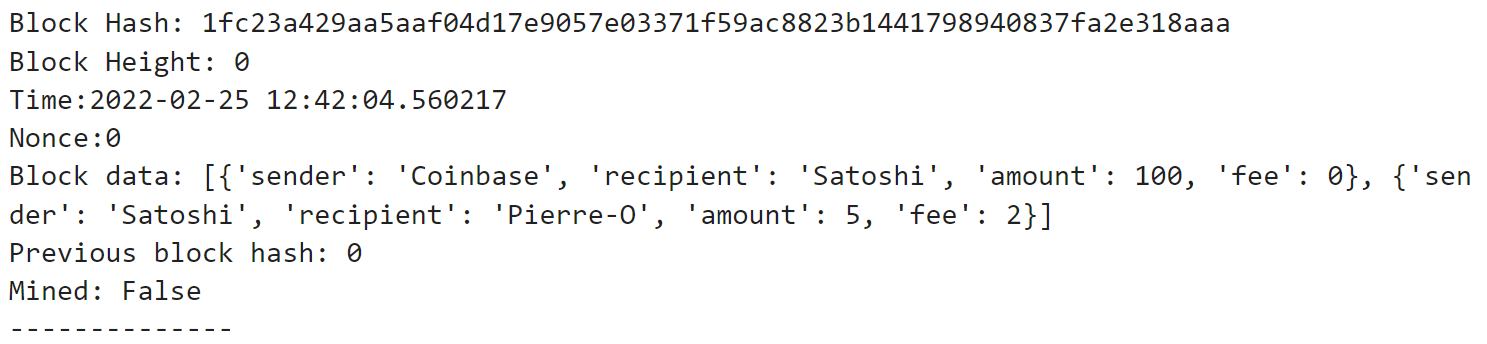
\includegraphics[width = \textwidth]{../../Figures/block_not_mined.png}
    \captionsetup{width=0.8\textwidth}
    \centering
    \caption{A block that has not been mined yet.}
    \label{fig:block_not_mined}
\end{figure}
\end{frame}
\begin{frame}{Mining a block}
The maximum value for a 256 bits number is
$$
T_\text{max} = 2^{256}-1 \approx 1.16e^{77}.
$$
Mining consists in drawing at random a nonce 
$$
\text{Nonce} \sim \text{Unif}(\{0,\ldots, 2^{32}-1\}),
$$
until 
$$
h(\text{Nonce}|\text{Block info})<T,
$$
where $T$ is referred to as the target.
\begin{tcolorbox}[enhanced,drop shadow, title=Difficulty of the cryptopuzzle]
$$
D = \frac{T_{\max}}{T}.
$$
\end{tcolorbox}

\end{frame}
\begin{frame}{Mining a block}
If we set the difficulty to $D = 2^4$ then the hexadecimal digest must start with at least $1$ leading $0$
\begin{figure}[!ht]
    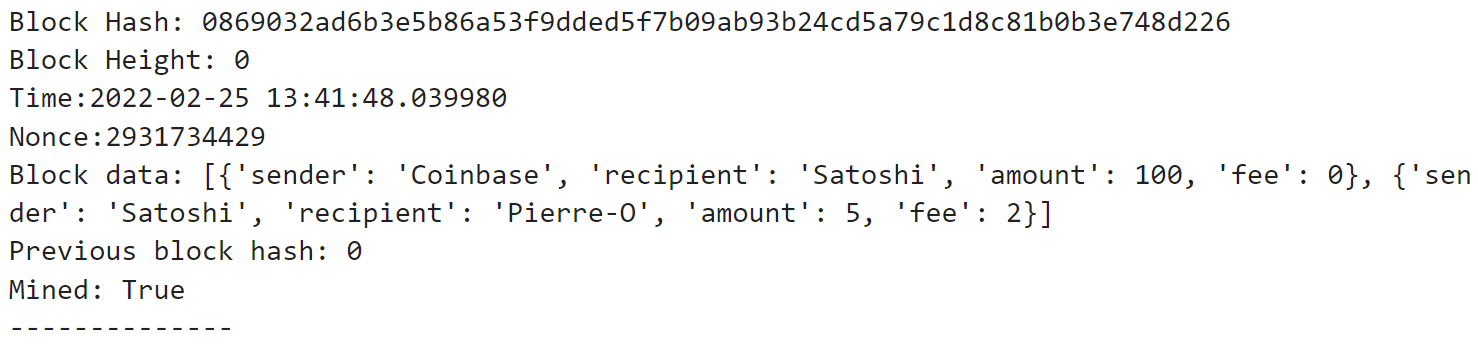
\includegraphics[width = \textwidth]{../../Figures/block_mined.png}
    \captionsetup{width=0.8\textwidth}
    \centering
    \caption{A mined block with a hash value having on leading zero.}
    \label{fig:block_mined}
\end{figure}
The number of trial is geometrically distributed
\begin{itemize}
\item Exponential inter-block times
\item Lenght of the blockchain = Poisson process
\end{itemize}
\end{frame}
\begin{frame}{Bitcoin protocol}
\begin{itemize}
  \item One block every 10 minutes on average
  \item Depends on the hashrate of the network
  \item Difficulty adjustment every 2,016 blocks ($\approx$ two weeks)
  % \item Reward halving every 210,000 blocks
\end{itemize}
% Check out \url{https://www.bitcoinblockhalf.com/}
\begin{tcolorbox}[enhanced,drop shadow, title=Risky business]
Steady operational cost VS infrequent capital gains
\end{tcolorbox}
\end{frame}

% \section{Insurance risk theory}
% \begin{frame}{Cramer-Lunberg risk model}
% \begin{columns}
% \begin{column}{0.5\textwidth}
% \scriptsize
% The financial reserves of a nonlife insurance company is given by
% \begin{equation*}
% R_t = u +ct - \sum_{i = 1}^{N_t}U_i\text{, }t\geq0,
% \end{equation*}
% où 
% \begin{itemize}
%   \item $u>0$ the initial reserves
%   \item $c$ is the premium rate
%   \item $(N_t)_{t\geq0}$ is the claim frequency up to time $t\geq0$.
%   \begin{itemize}
%     \scriptsize
%     \item[$\hookrightarrow$]  Poisson process with intensity $\lambda$
%   \end{itemize}
%   \item The $U_i$'s are the claim amounts
%   \begin{itemize}
%     \scriptsize
%     \item[$\hookrightarrow$] Nonnegative random variables, \textbf{i.i.d.}, and independent from $N_t$
%   \end{itemize}
% \end{itemize}
% \end{column}
% \begin{column}{0.5\textwidth}
% \begin{tikzpicture}
%   %Origin and axis
%   \coordinate (O) at (0,0);
%   \draw[->] (-0.5,0) -- (5.5,0) coordinate[label = {below:\scriptsize$t$}] (xmax);
%   \draw[->] (0,-0.5) -- (0,4) coordinate[label = {right:\scriptsize$R_t$}] (ymax);
%    %Initial reserves
%   \draw (0,2) node[black,left] {\scriptsize$u$} node{};
%  % % %Length of the honest chain
%   \draw[thick, tublue,-] (0,2) -- (2,3) node[pos=0.5, above] {};
%   \draw[thick, dashed, tublue] (2,3) -- (2,1) node[pos=0.5, left] {\scriptsize\color{black}$U_1$};
%   \draw[thick, tublue] (2,1) -- (3,1.5) node[pos=0.5, above] {};
%   \draw[thick, dashed, tublue] (3,1.5) -- (3, 0.5) node[pos=0.5, left] {\scriptsize\color{black}$U_2$};
%   \draw[thick, tublue] (3,0.5) -- (5, 1.5) node[pos=0.5, above] {};
%    \draw[thick, dashed, tublue] (5,1.5) -- (5, -0.5) node[pos=0.5,above left] {\scriptsize\color{black}$U_3$};

%   %Block finding Times 
%   \draw (2,0) node[black,below] {\scriptsize$T_1$} node{ \color{black}$\bullet$};
%   \draw (3,0) node[black,below] {\scriptsize$T_2$} node{ \color{black}$\bullet$};
%   \draw (5,0) node[black,below left] {\scriptsize$\tau_u$} node{ \color{black}$\bullet$};
% \end{tikzpicture}
% \end{column}
% \end{columns}

% \end{frame}
% \begin{frame}{Ruin probability}
% \scriptsize
% Define the ruin time as
% $$
% \tau_u = \inf\{t\geq0\text{ ; }R_t <0\}
% $$
% and the ruin probability as
% $$
% \psi(u,t) = \mathbb{P}(\tau_u < t)\text{ et }\psi(u) = \mathbb{P}(\tau_u < \infty)
% $$
% Find $u$ such that 
% $$
% \mathbb{P}(\text{Ruin}) = \alpha\text{ (0.005)},
% $$
% with
% $$
% c=(1+\eta)\lambda\mathbb{E}(U),
% $$
% where 
% $$\eta>0\text{ (net profit condition)}$$  
% otherwise 
% $$\psi(u)=1.$$

% \tiny
% \begin{thebibliography}{1}

% \bibitem{Asmussen_2010}
% S.~Asmussen and H.~Albrecher, {\em Ruin Probabilities}.
% \newblock {WORLD} {SCIENTIFIC}, sep 2010.

% \end{thebibliography}

% \end{frame}


\section{Blockchain miner's risk model}
\begin{frame}{Dual risk model}
\begin{columns}
\begin{column}{0.5\textwidth}
\scriptsize
Consider a miner 
\begin{itemize}
  \item of hashrate $p\in(0,1)$
  \item that owns $u\geq0$ at $t = 0$ 
  \item spends $c = \pi_W\cdot W\cdot p$ per time unit  
  \item who finds $p \lambda$ blocks on average per time unit, where $\lambda$ is the average number of blocks found by the network
\end{itemize}
The wealth of such a miner is given by
$$
R_t = u - c\cdot t + N_t\cdot b,\text{ (Dual risk model)}
$$
où 
\begin{itemize}
  \item $(N_t)_{t\geq0}$ is a Poisson process with intensity $p\cdot\lambda$
  \item $b$ is the block finding reward (6.25 BTC) \url{bitcoinhalf.com}
\end{itemize}
\end{column}
\begin{column}{0.5\textwidth}
\begin{tikzpicture}
  %Origin and axis
  \coordinate (O) at (0,0);
  \draw[->] (-0.5,0) -- (5.5,0) coordinate[label = {below:\scriptsize$t$}] (xmax);
  \draw[->] (0,-0.5) -- (0,4) coordinate[label = {right:\scriptsize$R_t$}] (ymax);
   %Initial reserves
  \draw (0,3) node[black,left] {\scriptsize$u$} node{};
 % % %Length of the honest chain
  \draw[thick, tublue,-] (0,3) -- (2,1) node[pos=0.5, above] {};
  \draw[thick, dashed, tublue] (2,1) -- (2,2) node[pos=0.5, above left] {\scriptsize\color{black}$b$};
  \draw[thick, tublue] (2,2) -- (3.5,0.5) node[pos=0.5, above] {};
  \draw[thick, dashed, tublue] (3.5,0.5) -- (3.5, 1.5) node[pos=0.5, above left] {\scriptsize\color{black}$b$};
  \draw[thick, tublue] (3.5,1.5) -- (5, 0) node[pos=0.5, above] {};

  %Block finding Times 
  \draw (2,0) node[black,below] {\scriptsize$T_1$} node{ \color{black}$\bullet$};
  \draw (3.5,0) node[black,below] {\scriptsize$T_2$} node{ \color{black}$\bullet$};
  \draw (5,0) node[black,below] {\scriptsize$\tau_u$} node{ \color{black}$\bullet$};
\end{tikzpicture}
\end{column}
\end{columns}
\end{frame}
\begin{frame}{Expected profit if no failure}
\scriptsize

The ruin time is defined as
$$
\tau_u  = \inf\{t\geq0\text{ ; }R_t \leq0\}
$$
\begin{itemize}
  \item Risk measure
  $$
  \psi(u,t) = \mathbb{P}(\tau_u \leq t)
  $$
  \item Profitability measure
  $$
  V(u,t) = \mathbb{E}(R_t\mathbb{I}_{\tau_u > t})
  $$
\end{itemize} 
\end{frame}
\begin{frame}{A miner's dilemma} 
\scriptsize
Use $\psi$ and $V$ to compare mining solo to
\begin{itemize}
  \item pool mining
\tiny
  \begin{thebibliography}{1}

\bibitem{rosenfeld2011analysis}
M.~Rosenfeld, ``Analysis of bitcoin pooled mining reward systems,'' 2011.

\bibitem[Albrecher et~al.(2022)Albrecher, Finger, and Goffard]{Albrecher2022}
Hansjörg Albrecher, Dina Finger, and Pierre-O. Goffard.
\newblock Blockchain mining in pools: Analyzing the trade-off between
  profitability and ruin.
\newblock \emph{Insurance: Mathematics and Economics}, 105:\penalty0 313--335,
  jul 2022.
\newblock \url{10.1016/j.insmatheco.2022.04.004}.
\end{thebibliography}
  \item \scriptsize deviating from the prescribed protocol (selfish mining)

  \tiny
  \begin{thebibliography}{1}
  \bibitem{Eyal2014}
I.~Eyal and E.~G. Sirer, ``Majority is not enough: Bitcoin mining is
  vulnerable,'' in {\em Financial Cryptography and Data Security},
  pp.~436--454, Springer Berlin Heidelberg, 2014.

\bibitem[Albrecher and Goffard(2022)]{Hansjoerg2022}
Hansjoerg Albrecher and Pierre-Olivier Goffard.
\newblock On the profitability of selfish blockchain mining under consideration
  of ruin.
\newblock \emph{Operations Research}, 70(1):179--200, jan
  2022.
\newblock \url{10.1287/opre.2021.2169}.
\end{thebibliography}
\end{itemize}
Analytical expressions for 
$$
\widehat{\psi}(u,t)= \mathbb{E}[\psi(u,T)]\text{ and }\widehat{V}(u,t)= \mathbb{E}[V(u,T)],
$$
where $T\sim\text{Exp}(t)$.
\end{frame}

\begin{frame}{Solo mining}
\scriptsize
\begin{tcolorbox}[enhanced,drop shadow, title=Theorem (profit and ruin when mining solo)]
For $u\geq0$, with 
\begin{equation*}
\widehat{\psi}(u,t) = e^{\rho^\ast u},
\end{equation*}
and 
\begin{equation*}
\widehat{V}(u,t) = u+(p\lambda b-c)t\left(1-e^{\rho^\ast u }\right),
\end{equation*}
where $\rho^\ast$ is the only nonnegative solution of
\begin{equation}\label{eq:equation_rho}
-c\rho + p\lambda(e^{b\rho}-1) = 1/t.
\end{equation}
\end{tcolorbox}
\begin{tcolorbox}[enhanced,drop shadow, title=Lambert function]
The solution $\rho^\ast$ of \eqref{eq:equation_rho} is given by 
\begin{equation*}
  \rho^{\ast}=-\frac{p \lambda t+1}{ct}
  -\frac{1}{b} \,{\rm W} \left[-\frac{p\lambda
    \,b}{c}\,{e^{-b\,\left(\frac{p \lambda t+1}{ct}\right)}}
  \right],
  \end{equation*}
  where $W(.)$ denotes the Lambert function.
\end{tcolorbox}
\end{frame}

\begin{frame}{Mining pool?}
\scriptsize
Let $I\subset\{1,\ldots, n\}$ be a set of miners with cumulated hashpower
$$
p_I = \sum_{i\in I }p_i,
$$
\begin{itemize}
  \item A pool manager coordinates the joint effort
  \item Miners show their work by submitting partial solutions (\textit{share})  
\end{itemize}
The pool manager chooses
\begin{itemize} 
  \item the participant remuneration system
  \item the relative difficulty $q\in(0,1)$ of finding a \textit{share} VS finding a proper solution
  \item the amount of management fees $f$
  \end{itemize} 
\end{frame}
\begin{frame}{Remuneration system}
\scriptsize
Miners must be compensated pro-rata to their contribution to the mining effort. 
\begin{tcolorbox}[enhanced,drop shadow, title=Proportional scheme]
A \text{round} is the time elapsed between two block discovery 
\begin{itemize} 
  \item $s_i$ is the number of \textit{shares} submitted by $i\in I$ during the \textit{round}
  \item Each miner receives 
  $$
  (1-f)\cdot b\cdot\frac{s_i}{\sum_{i\in I}s_i},
  $$
  at the end the round, where $f$ is the pool manager's cut.
  \item The system is deemed fair if $\frac{s_i}{\sum_{i\in I}s_i}\approx\frac{p_i}{\sum_{i\in I}p_i}$
\end{itemize}

\end{tcolorbox}
\end{frame}
\begin{frame}{What's wrong about going proportional}
\scriptsize
\begin{tcolorbox}[enhanced,drop shadow, title=Remarque]
This scheme is not incentive compatible
\end{tcolorbox}
\tiny
\begin{thebibliography}{1}

\bibitem{Schrijvers2017}
O.~Schrijvers, J.~Bonneau, D.~Boneh, and T.~Roughgarden, ``Incentive
  compatibility of bitcoin mining pool reward functions,'' in {\em Financial
  Cryptography and Data Security}, pp.~477--498, Springer Berlin Heidelberg,
  2017.

\end{thebibliography}
\scriptsize

\begin{itemize}
  \item The duration of \textit{rounds} is random 
  \begin{itemize}
    \scriptsize
    \item[$\hookrightarrow$] A \textit{share} loses value when the \textit{round} last for too long $\Rightarrow$ \textit{pool hoping} \tiny
    \begin{thebibliography}{1}

\bibitem{rosenfeld2011analysis}
M.~Rosenfeld, ``Analysis of bitcoin pooled mining reward systems,'' 2011.

\end{thebibliography}
\scriptsize
    \item[$\hookrightarrow$] Apply a discount factor to \textit{shares} \tiny
    \begin{thebibliography}{1}
\bibitem{slush}
slush pool, ``Reward system specifications,'' 2021.
\end{thebibliography}
  \end{itemize}
  \item A miner may postpone the communication of a solution
  \begin{itemize}
    \scriptsize
    \item[$\hookrightarrow$] to wait for her proportion of submitted \textit{shares} to improve 
  \end{itemize} 
  \item No risk transfer from miner to pool manager
    \begin{itemize}
    \scriptsize
    \item[$\hookrightarrow$] $f$ must be small
  \end{itemize} 
\end{itemize}

\end{frame}
\begin{frame}{The Pay-per-Share (PPS) system}
\scriptsize
The manager pays
$$
w = (1-f)\cdot q \cdot b 
$$ 
for every \textit{share} and keeps the block finding reward.\blfootnote{\url{https://en.bitcoin.it/wiki/Comparison_of_mining_pools}}
\vspace{1cm}
\begin{columns}
\begin{column}{0.5\textwidth}
Miner's wealth
$$
R_t^i = u_i-ct + M_t^i w,\text{ }t\geq0.
$$
where 
\begin{itemize}
   \item $(M_t^i)_{t\geq0}$ is a Poisson process with intensity $p_i \mu= p_i\lambda / q$
   \item $\mu$ is the average number of \textit{shares} submitted by the network
\end{itemize}
\end{column}
\begin{column}{0.5\textwidth}
Manager's wealth
$$
R_t^I = u_I - M_t^I w+N_t^I b,\text{ }t\geq0.
$$
where 
\begin{itemize}
   \item $(M_t^I)_{t\geq0}$ is a Poisson process with intensity $p_I\mu =p_I\lambda / q$
   \item $(N_t^I)_{t\geq0}$ is a Poisson process with intensity $p_I\lambda$
\end{itemize}
\end{column}
\end{columns}
\end{frame}
% \begin{frame}{Pool manager's risk}
% \scriptsize
% Let us consider randomized rewards
% $$
% R_t= u - \sum_{i=1}^{M_t} W_i +\sum_{j=1}^{N_t} B_j,\text{ }t\geq0.
% $$
% where
% \begin{itemize}
%   \item $(M_t)_{t\geq0}$ and $(N_t)_{t\geq0}$ are Poisson processes with intensity $\mu^\ast=\mu- \lambda$ and $\lambda$
%   \item $(W_i)_{i\geq0}$ and $(B_j)_{j\geq0}$ are two independent sequence of \iid exponential random variables with mean $w$ and $b^\ast = b-w$.
% \end{itemize}
% \begin{tcolorbox}[enhanced,drop shadow, title=Poisson process superposition]
% A block discovery triggers the payment of a \textit{share} to the miners
% \begin{itemize}
% \item The intensity of $M_t$ is given by $\mu^\ast=\mu- \lambda$ 
% \item The block finding reward is then $b^\ast = b-w$ 
% \end{itemize}
% A distinction is made here between jumps up and down.
% \end{tcolorbox}
% \end{frame}
\begin{frame}{Pool manager's risk}
\scriptsize
\begin{tcolorbox}[enhanced,drop shadow, title=Theorem (Profits and loss of a pool manager)]
The ruin probability is given by
\begin{equation*}\label{psiexpe}
    \widehat{\psi}(u,t) = (1-Rw)  e^{-R u},\;u\ge 0,
\end{equation*}
and the expected wealth is
\begin{equation*}\label{Vcombexpe}
    \w{V}(u,t) = (1 - Rw)[w-t(\lambda b^\ast-\mu^\ast w)] e^{-R u}+u+t(\lambda b^\ast-\mu^\ast w),
\end{equation*}
where $R$ is the only solution to 
\begin{equation*} \label{VLunde}
    -(t^{-1}+\lambda+\mu^\ast)+\lambda(1+b^\ast r)^{-1}+\mu^\ast(1-wr)^{-1}=0,
\end{equation*}
with positive real part.
\end{tcolorbox}
\tiny
  \begin{thebibliography}{1}

\bibitem{albrecher2021blockchain}
H.~Albrecher, D.~Finger, and P.-O. Goffard, ``Blockchain mining in pools:
  Analyzing the trade-off between profitability and ruin,'' 2021.


\end{thebibliography}
\end{frame}
\begin{frame}{Problem related to mining pools}
\begin{itemize}
  \item Arm race, ramping electricity consumption and e-waste generation
\tiny
\begin{thebibliography}{1}

\bibitem{bertucci2020mean}
C.~Bertucci, L.~Bertucci, J.-M. Lasry, and P.-L. Lions, ``Mean field game
  approach to bitcoin mining,'' 2020.

\bibitem{Alsabah2018}
H.~Alsabah and A.~Capponi, ``Bitcoin mining arms race: R{\&}d with
  spillovers,'' {\em {SSRN} Electronic Journal}, 2018.

\end{thebibliography}
\end{itemize}
\begin{itemize}
  \item \normalsize A threat on decentralization?\blfootnote{\url{https://btc.com/stats/pool?pool_mode=year}}
\tiny
\begin{thebibliography}{1}

\bibitem{Cong2020}
L.~W. Cong, Z.~He, and J.~Li, ``Decentralized mining in centralized pools,''
  {\em The Review of Financial Studies}, vol.~34, pp.~1191--1235, apr 2020.

\bibitem{li2019mean}
Z.~Li, A.~M. Reppen, and R.~Sircar, ``A mean field games model for
  cryptocurrency mining,'' 2019.
\end{thebibliography}
\end{itemize}
% \cite{Albrecher2022}
\end{frame}
% \begin{frame}
% \cite{albrecher:hal-03336851,Hansjoerg2022}
% \bibliography{../../blockastics}
% \bibliographystyle{plainnat}
% \end{frame}

\appendix
\begin{frame}{Solo mining}
\scriptsize
\begin{tcolorbox}[enhanced,drop shadow, title=Theorem (profit and ruin when mining solo)]
For $u\geq0$, with 
\begin{equation*}
\widehat{\psi}(u,t) = e^{\rho^\ast u},
\end{equation*}
and 
\begin{equation*}
\widehat{V}(u,t) = u+(p\lambda b-c)t\left(1-e^{\rho^\ast u }\right),
\end{equation*}
where $\rho^\ast$ is the only nonnegative solution of
\begin{equation}\label{eq:equation_rho}
-c\rho + p\lambda(e^{b\rho}-1) = 1/t.
\end{equation}
\end{tcolorbox}
\begin{tcolorbox}[enhanced,drop shadow, title=Lambert function]
The solution $\rho^\ast$ of \eqref{eq:equation_rho} is given by 
\begin{equation*}
  \rho^{\ast}=-\frac{p \lambda t+1}{ct}
  -\frac{1}{b} \,{\rm W} \left[-\frac{p\lambda
    \,b}{c}\,{e^{-b\,\left(\frac{p \lambda t+1}{ct}\right)}}
  \right],
  \end{equation*}
  where $W(.)$ denotes the Lambert function.
\end{tcolorbox}
\end{frame}
\begin{frame}{Sketch of the proof}
\scriptsize
The time-horizon is random with $T\sim\text{Exp}(t)$, we condition upon the events occuring in $(0,h)$, with $h<u/c$ so that ruin cannot occur before $h$. Three possibilities
\begin{itemize}
  \item[(i)] $T>h$ and no blocks $(0,h)$
  \item[(ii)] $T<h$ and no blocks $(0,T)$
  \item[(iii)] One block found before $T$ and $h$
\end{itemize}
The expected profit $\widehat{V}(u,t)$ satisfies
\begin{eqnarray*}
  \widehat{V}(u,t)& =&e^{-h(1/t + p\lambda)}\,\widehat{V}(u-ch,t)+\int\limits_0^h\frac1t\, e^{-s(1/t + p\lambda)}\,(u-cs)ds\\
  &+&\int\limits_0^h p\lambda\, e^{-s(1/t + p\lambda)}\,\widehat{V}(u-cs+b,t)ds.
  \end{eqnarray*}
  \end{frame}
\begin{frame}{Sketch of the proof}
\scriptsize
Differentiating with respect to $h$ and setting $h=0$, we get
\begin{equation}\label{eq:ODE}
c\widehat{V}'(u,t) + \left(\frac{1}{t} +  p\lambda\right)\widehat{V}(u,t) - p\lambda \widehat{V}(u+b,t) - \frac{u}{t} =0,
\end{equation}
Equation \eqref{eq:ODE} is an advanced differential equation
\blfootnote{\tiny 
 H.~L. Smith, {\em An introduction to delay differential equations with
  applications to the life sciences}.
\newblock Springer, New York, 2011.
}
with boundary conditions
$$
\widehat{V}(0,t) = 0 \text{ such that } 0\leq \widehat{V}(u,t)\leq u-ct+p\lambda b t \text{ for }u>0.
$$  
Consider solutions of the form 
\begin{equation}\label{eq:potential_solution}
\widehat{V}(u,t) = Ae^{\rho u }+Bu + C,\text{ }u \ge 0, 
\end{equation}
where $A, B,C$ and $\rho$ are constants to be determined. Substituting \eqref{eq:potential_solution} in \eqref{eq:ODE} together with boundary conditions
\begin{equation*}
\begin{cases}
0&=ct\rho + \left(1+p\lambda t\right)-p\lambda te^{\rho b}, \\
0&= B\left(1+tp\lambda\right)-p\lambda tB - 1,\\
0&=Bct+C(1+tp\lambda) - p\lambda t Bb-p\lambda tC, \\
0&=A+C.
\end{cases}
\end{equation*}
\end{frame}
\begin{frame}{Sketch of the proof}
\scriptsize
We get $A = -t(p\lambda b - c)$, $B = 1$, $C = t(p\lambda b - c)$ and $\rho$ verifies
$$
c\rho + \left(1+p\lambda t\right)-p\lambda te^{\rho b} = 0,
$$
The latter has two solutions on the real line, one negative and the other is positive. As $A<0$, we must take  $\rho^\ast<0$ to ensure that $\widehat{V}(u,t)>0$. Substituting $A,B,C$ and $\rho^{\ast}$ in \eqref{eq:potential_solution} yields the result.\\

Similarly, the ruin probability satisfies
\begin{equation*}\label{psii}
c\widehat{\psi}'(u,t)+(p \lambda+1/t)\,\widehat{\psi}(u,t)-p \lambda\,\widehat{\psi}(u+b,t)=0
\end{equation*}
with initial condition $\widehat{\psi}(0,t)=1$ and boundary condition $\lim_{u\to\infty}\widehat{\psi}(u,t)=0$.
\end{frame}
\begin{frame}{Pool manager's risk}
\scriptsize
\begin{tcolorbox}[enhanced,drop shadow, title=Theorem (Profits and loss of a pool manager)]
The ruin probability is given by
\begin{equation*}\label{psiexpe}
    \widehat{\psi}(u,t) = (1-Rw)  e^{-R u},\;u\ge 0,
\end{equation*}
and the expected wealth is
\begin{equation*}\label{Vcombexpe}
    \w{V}(u,t) = (1 - Rw)[w-t(\lambda b^\ast-\mu^\ast w)] e^{-R u}+u+t(\lambda b^\ast-\mu^\ast w),
\end{equation*}
where $R$ is the only solution to 
\begin{equation*} \label{VLunde}
    -(t^{-1}+\lambda+\mu^\ast)+\lambda(1+b^\ast r)^{-1}+\mu^\ast(1-wr)^{-1}=0,
\end{equation*}
with positive real part.
\end{tcolorbox}
\tiny
  \begin{thebibliography}{1}

\bibitem{albrecher2021blockchain}
H.~Albrecher, D.~Finger, and P.-O. Goffard, ``Blockchain mining in pools:
  Analyzing the trade-off between profitability and ruin,'' 2021.


\end{thebibliography}
\end{frame}
\begin{frame}[allowframebreaks]{Sketch of the proof}
\scriptsize
Conditionning upon the events that occur during $(0,h)$. Four possibilities
\begin{itemize}
  \item[(i)] $T>h$ and no jumps $(0,h)$
  \item[(ii)] $T<h$ and no jumps $(0,T)$
  \item[(iii)] an upward jump $(0,h)$
  \item[(iv)] a downward jump $(0,h)$
\end{itemize}
  \begin{eqnarray*}\label{neu0}
      \w{V}(u,t)&=& e^{-(\frac{1}{t}+\lambda+\mu^\ast)h}\w{V}(u,t) + \frac{1}{t}\int_0^h e^{-{s}/{t}}e^{-(\lambda +\mu^\ast) s} u\,ds\\
      & +& \lambda\int_0^he^{-\lambda s} e^{-({1}/{t}+\mu^\ast) s} \int_0^\infty\w{V}(u+x,t)\,dF_{B}(x)\,ds\\
      &  +&\mu^\ast \int_0^he^{-\mu^\ast s} e^{-({1}/{t}+\lambda) s}\int_0^u \w{V}(u-y,t) \,dF_W(y)\,ds.
  \end{eqnarray*}
  Differentiating with respect to $h$ and letting $h\rightarrow 0$, yields
  \begin{equation} \label{inteq}
    \lambda\int_0^\infty\w{V}(u+x,t)\,dF_{B}(x)-(\lambda+\mu^\ast+{1}/{t})\w{V}(u,t)+\mu^\ast\int_0^u \w{V}(u-y,t) \,dF_W(y)+{u}/{t}=0,\quad u\ge 0,
  \end{equation}
  with boundary conditions $\w{V}(u,t)=0$ pour tout $u<0$ et $0\leq\w{V}(u,t)\leq u+(\lambda b^\ast - \mu^\ast w)t$. Consider solutions of the form
  $$
  Ce^{-ru}+d_1u+d_0
  $$
  \begin{itemize}
    \item Gathering the terms in factor of $e^{-r u}$ yields an equation for $r$ with
    $$
    -(t^{-1}+\lambda+\mu^\ast)+\lambda(1+b^\ast r)^{-1}+\mu^\ast(1-wr)^{-1}=0
    $$
    with nonnegative solution $R>0$, negative is impossible because $0\leq\w{V}(u,t)\leq u+(\lambda b^\ast - \mu^\ast w)t$
    \item Gathering the terms in factor of $u$, yields $d_1 = 1$
    \item Gathering the terms in factor of $1$, yields
    $$
    d_0 = t(\lambda b^\ast-\mu^\ast w)
    $$
    \item Gathering the terms in factor of $e^{-u/w}$, yields
    $$
    C = (1 - Rw)[w-t(\lambda b^\ast-\mu^\ast w)]
    $$
  \end{itemize}
\end{frame}
\end{document}
